\chapter{Materiais e Métodos} \label{cap:metod}

Nesse capítulo são descritos os métodos, assim como os materiais utilizados para o desenvolvimento deste trabalho. São descritas as etapas do projeto e os principais fundamentos e tecnologias a serem empregados.


\section{Materiais}
% arnaldo: 3.1 materiais: flutter, dart, python, mlkit, firebase, macbook para codificar (processador, memória, ...), software de emulação, iphone (geração, câmera, ...)
O ambiente de desenvolvimento da metodologia proposta se faz o uso de um Macbook Pro de 13 polegadas com processador Intel Core i5 de dois núcleos 2,3 GHz e memória integrada LPDDR3 de 8 GB com 2133 MHz e embarcado com o sistema operacional macOS Mojave versão 10.14.4.  

Para o desenvolvimento da metodologia, foi optado por utilizar as tecnologias de aplicativos móveis como Flutter, Dart e Firebase MLKit devido às suas altas taxas de aprendizado e desempenho no desenvolvimento de aplicativos móveis.

O Flutter\footnote{https://flutter.dev/} foi construído pela Google com a finalidade de melhorar a qualidade dos aplicativos, a velocidade do desenvolvimento, e para alcançar mais usuários. Ele é um SDK  de código aberto para o desenvolvimento de aplicativos para Desktop, Web e dispositivos móveis como iOS e Android \cite{ARSTECHNICA2017}.


O Flutter é um poderoso \textit{framework} porque o código é compilado em ARM, ou seja, compila o código para cada plataforma. Isso agiliza a abertura e o desempenho do aplicativo. Além disso, utiliza um renderizador Mobile First acelerado por GPU para que haja consistência da \textit{UI} entre as plataformas e o dispositivo. Então o Flutter projeta os \textit{widgets} com um \textit{framework} personalizável e extensível em camadas \cite{IMASTERS}. Não há pontes entre o \textit{framerwork} e os \textit{widgets}, tornando a renderização eficiente. 

Flutter é escrito em Dart, uma linguagem concisa, fortemente tipificada e orientada a objetos. O Dart é bem semelhante à linguagens como Swift, C#, Java e JavaScript.



Para a extração dos caracteres da imagem será utilizado o SDK Firebase ML Kit\footnote{https://firebase.google.com/}, após a etapa de pré-processamento será testado a eficácia tanto da sua versão \textit{online} quanto \textit{offline}, para uma taxa maior de acertos nas palavras, diminuindo a complexidade da busca pelos registros na base de dados da ANVISA, disponibilizada em seu \textit{site} oficial.

Os testes serão realizados por meio de um dispositivo físico Samsung J2 com processador de 1.4GHz, equipado com câmera traseira com resolução de 8.0 MP, lançado em outubro de 2015, um celular antigo e com recursos de memória e processamento limitados se comparados com celulares do ano de lançamento do desenvolvimento do presente trabalho, a fim de simular um caso extremo, porém possível de acontecer na sociedade.



% arnaldo: 3.2 método: criar base (capturar imagens, dizer quantas imagens,  resolução, colorido, iluminação);  pré-processar para tirar as bordas e corrigir a perspectiva; ocr; buscar na base; vai ter algum pos-processamento (ex. corretor ortográfico para contorar falhas do ocr)


\section{Coleta de imagens}

Foi necessário a realização da coleta de caixas de medicamentos para formar a base de imagens que possibilitaram os testes deste trabalho. Foram coletadas 6 caixas de medicamentos conforme a Figura \ref{exemplares}, com especificações diferentes, entre elas: proporções, fontes, cores e finalidade. Entre as caixas de medicamentos, apenas um medicamento entre os 6 não é regulamentado pela a Anvisa, o que foi um ponto importante para o desenvolvimento do aplicativo. Todas as caixas coletadas foram fornecidas pela farmácia Hiper Farma da cidade de Medianeira. Dessa maneira, foi possível ser construída a base de imagens.

 \begin{figure}[h!]
	\centering
	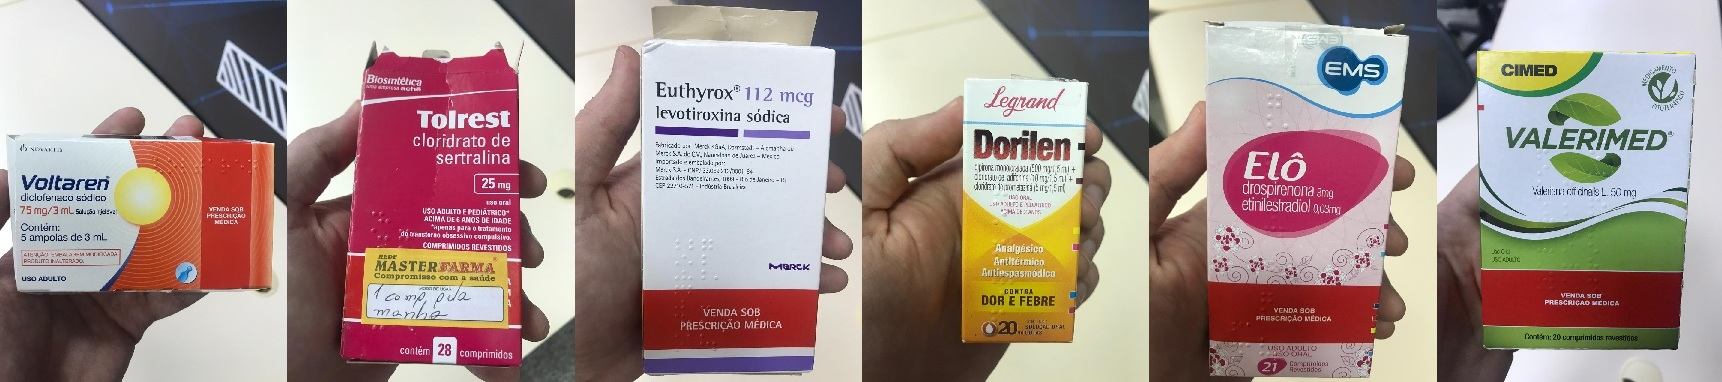
\includegraphics[width=0.99\textwidth]{Imagens/exemplares.jpg} 
	\caption[Exemplares de medicamentos utilizados.]{Exemplares de medicamentos utilizados.}
\fonte{Autoria própria.}
	\label{exemplares}
\end{figure}


A base de imagens é composta por 150 imagens com resolução de 3264x2448 \textit{pixel}, classificadas em 5 categorias, econforme a Tabela \ref{tab:catImg} e composta por imagens de 6 medicamentos, como descrito na próxima sessão.


\begin{table}[]
\caption{Categoria de imagens}
\label{tab:catImg}
\centering
\begin{tabular}{lcccc}
\hline
Nome da Categoria & Nome Abreviado & Tamanho (MB) & Quantidade de Imagens \\ \hline
Boa luminosidade & set1 & 76,8 MB & 30 \\
Baixa luminosidade & set2 & 104 MB & 30 \\
Ambiente externo & set3 & 88,9 MB & 30 \\
Noturnas sem flash & set4 & 82,9 MB & 30 \\
Noturnas com flash & set5 & 96,7 MB & 30 \\ \hline
\end{tabular}
\fonte{(Autoria Própria)}	
\end{table}



 
\subsection{Categorias da base de imagens}

 Todas as categorias são compostas por imagens de 6 medicamentos, onde cada medicamento possui 5 fotos em cada categoria. Cada foto foi capturada em uma diferente perspectiva, formando assim, 5 perspectivas demonstradas na Figura \ref{perspectiva}, que são:
   \begin{enumerate}
   \item Fotos chapadas, com a captura perpendicular ao plano de interesse da caixa.
   \item Fotos do topo, com inclinação média de 15 graus no topo em relação ao plano de interesse da caixa.
    \item Fotos da lateral esquerda, com inclinação aproximada de 15 graus na lateral esquerda em relação ao plano de interesse da caixa.
    \item Fotos da lateral direita, com inclinação média de 15 graus na lateral direita em relação ao plano de interesse da caixa.
    \item Fotos da base inferior, com inclinação média de 15 graus na base inferior em relação ao plano de interesse da caixa.
 \end{enumerate}
  \begin{figure}[h!]
	\centering
	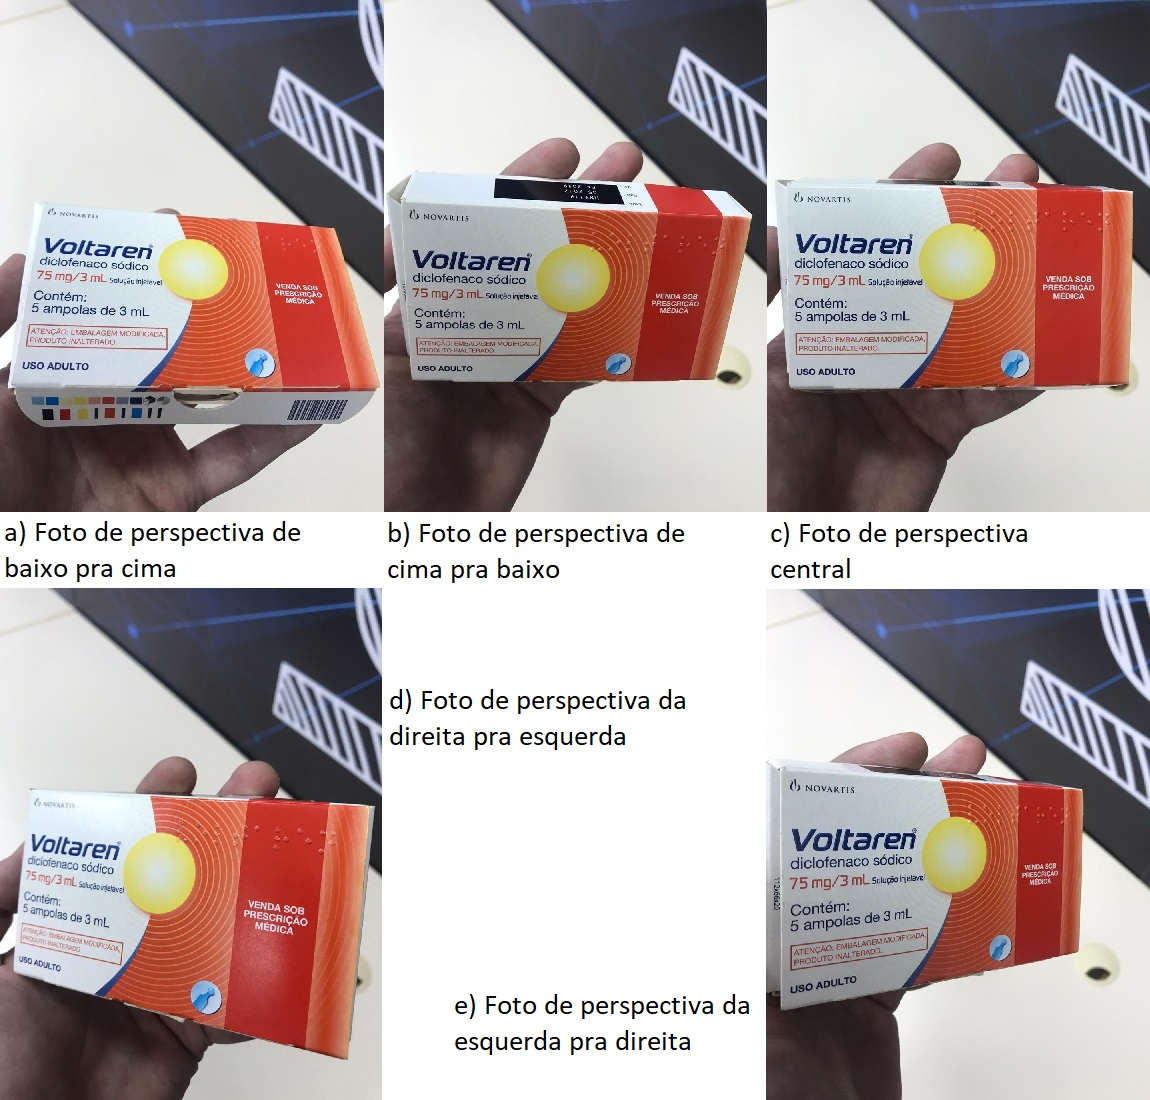
\includegraphics[height=0.70\textwidth]{Imagens/perspectiva.jpg} 
	\caption[Exemplar de medicamento em diferentes perspectivas.]{Exemplar de medicamento em diferentes perspectivas}
\fonte{Autoria própria.}
	\label{perspectiva}
\end{figure}
 
 



\section{Desenvolvimento do aplicativo}
Inicialmente, os aplicativos criados nesse trabalho foram desenvolvidos fazendo uso do \textit{framework} Flutter, como previstos na sessão de materiais. A versão utilizada para os experimentos foram as versões 1.9 do Flutter e 2.5 do Dart (linguagem utilizada pelo Flutter). O ambiente para o desenvolvimento foi \textit{Windows 10 64 bits} e a ferramenta específica para a implementação foi a \textit{IDE} Android Studio versão 3.5.
Os testes de execução da aplicação ocorreram em um dispositivo celular  modelo Samsung J2 Prime, portando um processador de 1.4 \textit{GHz Quad Core} e uma câmera traseira de 8 \textit{megapixel}. 

Para a configuração do \textit{plugin} que faz uso do OCR, foi utilizado o \textit{framework} Firebase MLKit para o reconhecimento de caracteres. Este \textit{framework} possui recursos para reconhecimento de imagens
\textit{online} e \textit{offline},
que permite ser feita a comparação do reconhecedor de caracteres, tanto online no servidor do \textit{framework}, quanto \textit{offline} no dispositivo.

O pacote de desenvolvimento do \textit{Firebase ML Vision} foi utilizado na versão 0.9.2, lançada em 23 de julho de 2019.	Utilizando o pacote de desenvolvimento do \textit{Firebase Vision}, é possível extrair o texto em 3 diferentes formas: em blocos, linha e palavras, todas com seu nível de confiança de 0 a 100 porcento, onde 0 porcento indica não confiável ao poder acertivo do OCR e 100 porcento significa total certeza de poder acertivo do OCR.
 
 Para armazenar os dados dos medicamentos extraídos do bulário da Anvisa, foi montado um modelo de arquivo JSON e importado manualmente os dados de cada medicamento.


\subsection{Processamento de imagem}
O presente trabalho faz uso de métodos de processamento de imagem com intuito de buscar um filtro que melhore o poder acertivo do OCR, possibilitando comparar os resultados finais que serão apresentados no tópico a seguir.

Os métodos propostos para a etapa de pré processamento são aplicadas às imagens originais. Ainda analisando a Figura \ref{tratamentoimg}, pode-se observar no centro, a imagem original, sem pré processamento de imagem em um ambiente considerado perfeito devido ao ambiente com boa luminosidade exposto. À esquerda da Figura \ref{tratamentoimg} está exposta a representação da imagem exposta ao algoritmo de efeito de Sobel e a direita é representada a imagem com efeito aplicado de escalas em cinza.

\begin{figure}[h!]
	\centering
	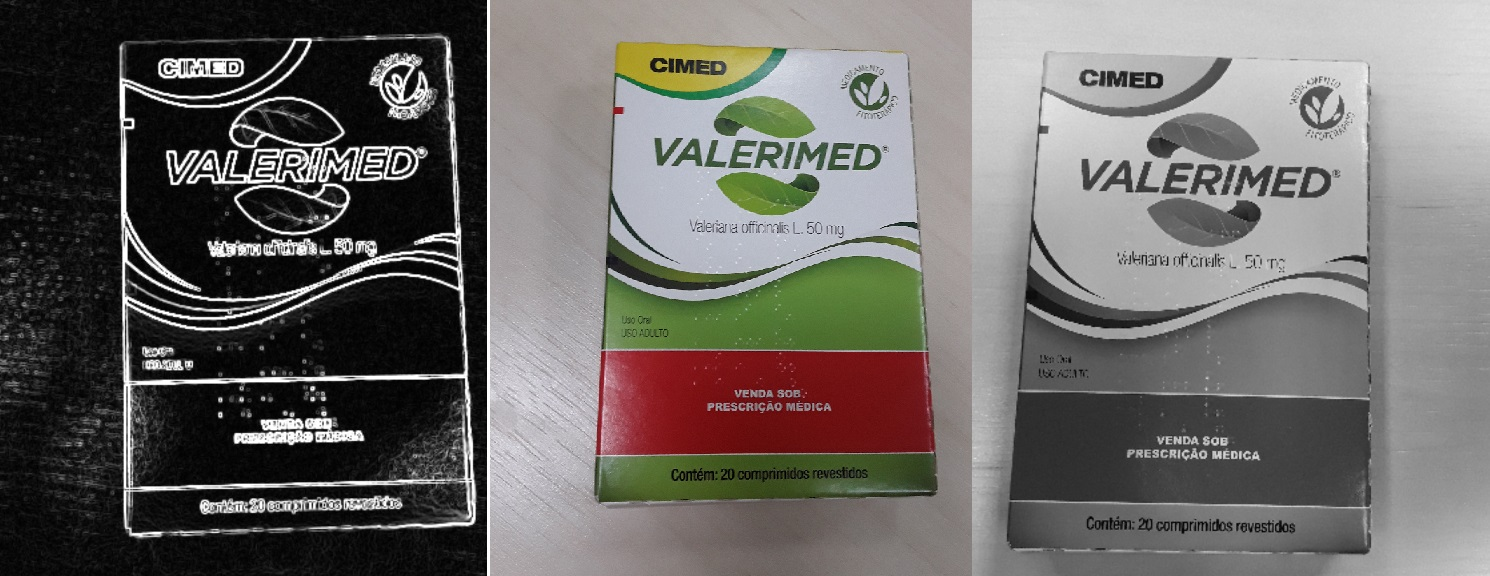
\includegraphics[width=0.90\textwidth]{Imagens/tratamentoimg.jpg} 
	\caption[Imagens expostas ao processamento de imagem.]{Imagens expostas ao processamento de imagem.}
\fonte{Autoria própria.}
	\label{tratamentoimg}
\end{figure}